\documentclass[12pt]{exam}
\usepackage[hon]{template-for-exam}
\usepackage{tikz,ifthen,multicol}
\footer{}{}{}
\header{}{}{}
\shadedsolutions
\printanswers
\usetikzlibrary{shadings,decorations.pathmorphing,arrows.meta,patterns}


\tikzstyle{box}=[rounded corners,draw,minimum height=1cm]


\begin{document}



\def\mystrut{\protect\rule[-2.2ex]{0ex}{2.2ex}} 
\qformat{ \textbf{Task \#\thequestion}
  \ifthenelse{\equal{\thequestion}{\thequestiontitle}}
    {}
    {: \emph{\thequestiontitle}}
  \mystrut  \hfill}
\begin{questions}

\large

\question
Consider a 1400-kg car that experiences 900 N of friction and 1300 N of air drag. How much force must the car's engine exert in order to maintain a constant speed of 45 m/s?

\begin{solution}
  2200 N
\end{solution}


\vs \hrule \vs

\question 

\hfill

\begin{multicols}{2}

  
  Two masses are suspended at rest.  Assume that $m_1=5.2$~kg and $m_2 = 1.7$~kg.

  \begin{parts}
    \part Draw a free-body diagram for each mass.
    \part Calculate the tension on each rope.
  \end{parts}
  \vs

  \begin{center}
    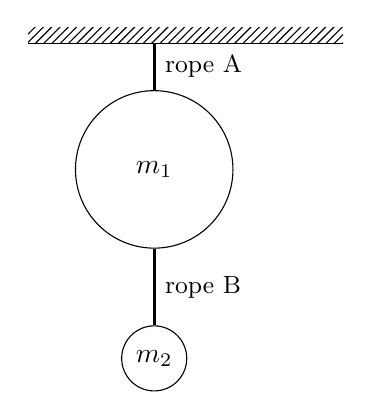
\begin{tikzpicture}[scale=0.8]
      \node[circle,draw,minimum size=2cm] (one) at (0,-2) {$m_1$};
      \node[circle,draw] (two) at (0,-5) {$m_2$};
      \draw[very thick] (one.south) -- (two.north) 
        node[midway,anchor=west] {\small rope B};
      \draw[very thick] (one.north) -- (0,0)
        node[midway,anchor=west] {\small rope A};
      \fill[pattern=north east lines] (-2,0) rectangle
        ++(5,0.25);
      \draw (-2,-0) -- ++(5,0);
    \end{tikzpicture}
  \end{center}
  
\end{multicols}




\begin{solution}
  $T_A=67.62$ N; $T_B=16.66$ N 
\end{solution}


\vs \hrule \vs

\question 

\hfill

\begin{multicols}{2}

  
  Now you've detached rope A and are accelerating the system upward at a rate of \SI{0.5}{m/s^2}, what would be the tensions on both ropes?


  \begin{parts}
    \part Draw a free-body diagram for each mass.
    \part Calculate the tension on each rope.
  \end{parts}
  \vs

  \begin{center}
    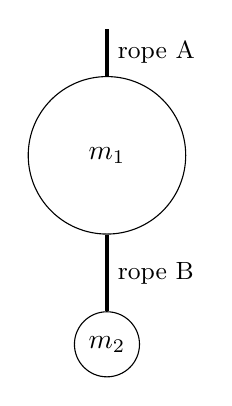
\begin{tikzpicture}[scale=0.8]
      \node[circle,draw,minimum size=2cm] (one) at (0,-2) {$m_1$};
      \node[circle,draw] (two) at (0,-5) {$m_2$};
      \draw[very thick] (one.south) -- (two.north) 
        node[midway,anchor=west] {\small rope B};
      \draw[very thick] (one.north) -- (0,0)
        node[midway,anchor=west] {\small rope A};

    \end{tikzpicture}
  \end{center}
  
\end{multicols}




\begin{solution}
  $T_A=71.07$ N; $T_B=17.51$ N 
\end{solution}


\pagebreak

\question
Two boxes have masses $m_1=20$ kg and $m_2=10$ kg and are sitting on a frictionless surface connected by a massless cord.  They are pulled with an applied force of $F=50$~N.
\begin{parts}
  \part Draw a free-body diagram for each mass. 
  \part Calculate the acceleration of the system. 
  \part Calculate the tension in the cord connecting them.
\end{parts}


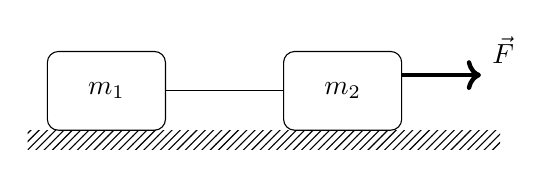
\begin{tikzpicture}
  \node[box,minimum width=1.5cm] (one) at (0,0) {$m_1$};
  \node[box,minimum width=1.5cm] (two) at (3,0) {$m_2$};
  \draw (one.east) -- (two.west);
  \draw[->,ultra thick] (two.east) ++(0,0.2) -- +(1,0) node[anchor=south west] {$\vec{F}$};
  \fill[pattern=north east lines] (-1,-0.5) rectangle ++(6,-0.25);
\end{tikzpicture}

\begin{solution}
  1.67 m/s$^2$; 16.7 N
\end{solution}



\vs \hrule \vs
  
\question
Two masses $m_1=4$ kg and $m_2=2$ kg are attached by a string that hangs over a frictionless pulley. What is (a) the tension on the string and (b) the acceleration of the masses? (This is known as an \emph{Atwood Machine})

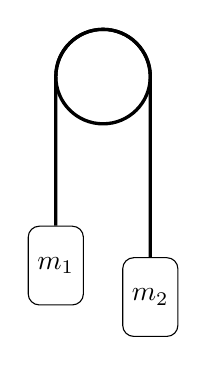
\begin{tikzpicture}[scale=0.8]
  \node[box] (one) at (-.75,0) {$m_1$};
  \node[box] (two) at (.75,-0.5) {$m_2$};
  \draw[very thick] (one.north) -- (-.75,3) 
    arc (180:0:.75) -- (two.north);
  \draw[very thick] (0,3) circle[radius=.75];
\end{tikzpicture}

\begin{solution}
  26.14 N; 3.27 m/s$^2$

  Extension: How much downward force would need to be applied on $m_2$ in order to keep the system from moving? (19.6 N)
\end{solution}

\vs \hrule \vs

\question
We now have what is called a \emph{Modified Atwood Machine} with $m_1=4$ kg and $m_2=3$ kg. What is (a) the tension on the string and (b) the acceleration of the masses? Again, the surface is frictionless.

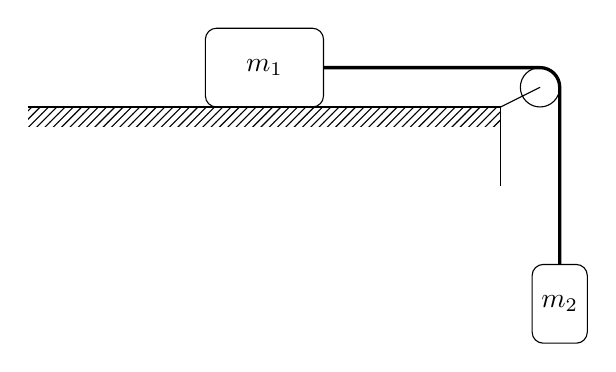
\begin{tikzpicture}
  \node[box,minimum width=1.5cm] (one) at (0,0) {$m_1$};
  \node[box] (two) at (3.75,-3) {$m_2$};
  \draw[very thick] (one.east) -- (3.5,0) arc (90:0:0.25) -- (two);
  \fill[pattern=north east lines] (-3,-0.5) rectangle
    ++(6,-0.25);
  \draw (-3,-0.5) -- 
    ++(6,0) coordinate (edge) -- 
    ++(0,-1);
  \draw (edge) -- (3.5,-0.25) circle (0.25);
\end{tikzpicture}

\begin{solution}
  
\end{solution}





\end{questions}

\end{document}